\newpage
\section{Routines}

    \subsection{Poisson Distribution}
        
        \begin{equation}
            P(k) = \frac{\mu^k e^{-\mu}}{k!}
            \label{eq:poisson}
        \end{equation}

        \lstinputlisting[language=Python, caption=poisson.py]{poisson.py}
        \lstinputlisting[language=Python]{output/poisson.txt}
        
        
    \newpage
    \subsection{Random Number Generator}
    
        \begin{equation}
            x_{j+1} = a x_{j} + c \mod m
            \label{eq:mlcg}
        \end{equation}
        
        \begin{equation}
            \begin{array}{l}
            x_{j+1} = x_{j} \land (x_{j} \ll a) \\
            x_{j+1} = x_{j} \land (x_{j} \gg b) \\
            x_{j+1} = x_{j} \land (x_{j} \ll c)
            \end{array}
            \label{eq:xor_shift}
        \end{equation}

        \lstinputlisting[language=Python, caption=RNG.py]{RNG.py}
        \lstinputlisting[language=Python]{output/RNG.txt}
        
        \begin{figure}[H]
            \centering
            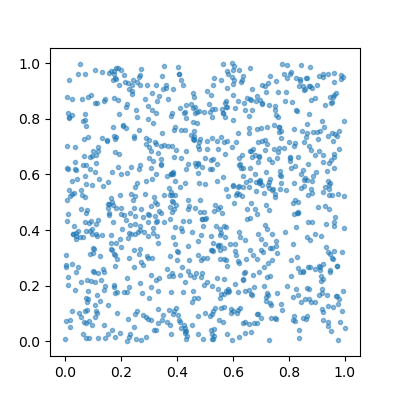
\includegraphics[height=6cm]{output/RNG_scatter.png}
            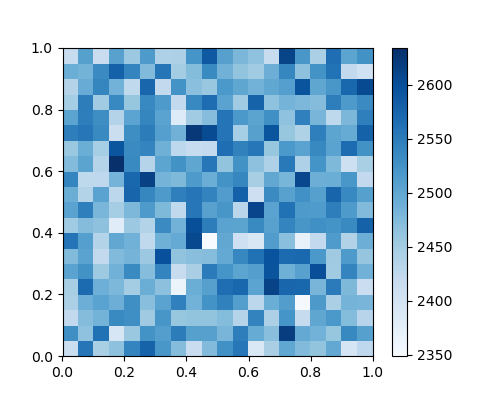
\includegraphics[height=6cm]{output/RNG_hist2d.png}
            \caption{The first thousand (left) and million (right) psuedo random numbers from the above generator. The coordinates of each point are given as  ($x_j$, $x_{j+1}$)}
            \label{fig:rng}
        \end{figure}
        